\documentclass{beamer}
\usepackage{mathtools}
\usepackage{xspace}
\usepackage{commath}

\let\arrowvec\vec
\renewcommand{\vec}[1]{\ensuremath{\mathbf{#1}}}
\newcommand{\integral}[1]{\ensuremath{\left\langle #1 \right\rangle}}
\newcommand{\closure}[1]{\ensuremath{\mathcal{E}(#1)}}
\newcommand{\T}[1]{\ensuremath{#1^\textnormal{T}}}
\newcommand{\R}{\ensuremath{\mathbb{R}}\xspace}
\newcommand{\SN}{\ensuremath{\textnormal{S}_\textnormal{N}}\xspace}
\newcommand{\PN}{\ensuremath{\textnormal{P}_\textnormal{N}}\xspace}
\newcommand{\MN}{\ensuremath{\textnormal{M}_\textnormal{N}}\xspace}
\newcommand{\PPN}{\ensuremath{\textnormal{PP}_\textnormal{N}}\xspace}
\newcommand{\FPN}{\ensuremath{\textnormal{FP}_\textnormal{N}}\xspace}
\newcommand{\DN}{\ensuremath{\textnormal{D}_\textnormal{N}}\xspace}
\newcommand{\kinetic}{\texttt{kinetic}\xspace}
\newcommand{\moment}{\texttt{moment}\xspace}
\newcommand{\momopt}{\texttt{momopt}\xspace}
\newcommand{\valpha}{\mbox{\boldmath$\alpha$}\xspace}

\usetheme{Madrid}
\beamertemplatenavigationsymbolsempty
\frenchspacing

\title{\texttt{closures-2d}}
\author{Tim Shaffer\thanks{Mentor: C. Kristopher Garrett}}

\begin{document}
    \frame{\titlepage}

    \begin{frame}{Goals}
        We are releasing software that tests angular approximations in kinetic transport simulations
        \begin{itemize}
            \item Based on code used for a previous publication~(citation)
            \item Open source so that others can use/collaborate
            \item Makes it easy to implement new features
            \item Implements \SN, \PN, \FPN, \MN, \PPN, \DN~(experimental)
        \end{itemize}

        [pictures]
    \end{frame}

    \begin{frame}{Improvements}
        Algorithmic changes:
        \begin{itemize}
            \item Added experimental Lebedev quadrature
            \item Removed $\gamma$ factor for ansatz correction in \texttt{momopt}
            \item Changed \texttt{momopt}'s regularization in case of bad condition number
        \end{itemize}

        \vfill

        Software-related improvements:
        \begin{itemize}
            \item Cross-platform build system
            \item Automated testing
            \item Better MPI communication
            \item Improved documentation
            \item Improved interface
            \item Bugfixes
            \item Profiling and optimization
        \end{itemize}
    \end{frame}

    \begin{frame}{Release}
        We are releasing this code as open source software.

        \vfill

        Now uses SCons, a Python-based build system, rather than Makefiles
        \begin{itemize}
            \item Cross platform
            \item Sets up library search paths
            \item Intelligent compilation
        \end{itemize}

        \vfill

        Depends on:
        \begin{columns}
            \column{0.25 \textwidth}
            \begin{itemize}
                \item GSL
                \item BLAS
                \item LAPACK
            \end{itemize}
            \column{0.4 \textwidth}
            \begin{itemize}
                \item OpenMP (optional)
                \item Open MPI (optional)
                \item PAPI (optional)
            \end{itemize}
        \end{columns}
    \end{frame}

    \begin{frame}[fragile=singleslide]{Testing}
        We implemented several automated tests for the software.
        The testing code is written in Python and integrated with the build system.

        \vfill

        The testing code carries out
        \begin{itemize}
            \item Regression tests -- compare output to reference data included with the software
            \item Mass Conservation tests -- check that total density remains the same
            \item Convergence tests -- measure the effect of decreasing the cell size on the precision of the output
        \end{itemize}

        \vfill

        \begin{verbatim}
convergence tests:
 - moment(sspline)
 -- dx / 16                      35.922s
 -- dx / 8                        4.580s
 -- dx / 4                        0.603s           2.340759
 -- dx / 2                        0.092s           2.082828
 -- dx / 1                        0.022s           1.954163
        \end{verbatim}
    \end{frame}


    \begin{frame}{Performance}
        Added timing and profiling-related measurement capabilities

        \vfill

        Tested additional optimizations
        \begin{itemize}
            \item Spatial blocking (reduce scheduling overhead, cache misses)
            \item CPU pinning (ccNUMA)
            \item Memory alignment
        \end{itemize}
    \end{frame}

    \begin{frame}{The Importance of Caching}
        
    \end{frame}

    \begin{frame}{Blocking}
        
    \end{frame}

    \begin{frame}{What Are Kinetic Equations?}
        \begin{columns}[t]
            \column{0.45 \textwidth}
            \begin{block}{Macroscopic}
                \begin{itemize}
                    \item $\rho(\vec{x},t)$ -- Density
                    \item $\vec{u}(\vec{x},t)$ -- Velocity
                    \item $E(\vec{x},t)$ -- Kinetic Energy
                \end{itemize}
                Discretize \vec{x}, $t$ into 100 values: 4GB memory requirement
            \end{block}
            \column{0.45 \textwidth}
            \begin{block}{Mesoscopic}
                \begin{itemize}
                    \item $f(\vec{x},\vec{v},t)$ -- Density with respect to space \emph{and velocity}
                \end{itemize}
                Discretize \vec{x}, \vec{v}, $t$ into 100 pieces: 800TB memory requirement
            \end{block}
        \end{columns}

        \vfill

        Macroscopic can be derived from mesoscopic
        \begin{itemize}
            \item $\rho(\vec{x},t) = \int_{\R^3} f \dif \vec{v}$
            \item $\vec{u}(\vec{x},t) = \frac{1}{\rho} \int_{\R^3} \vec{v}f \dif \vec{v}$
            \item $E(\vec{x},t) = \frac{1}{2} \int_{\R^3} \| \vec{v} - \vec{u} \|^2 \dif \vec{v}$
        \end{itemize}
    \end{frame}

    \begin{frame}{What Are Kinetic Equations?}
        First used for rarefied gas dynamics (e.g. high altitude gases where collisions do not dominate the physics)

        \[\partial_t f + \vec{v} \cdot \nabla_\vec{x} = C(f)\]
        where $\int C(f) \dif \vec{v} = 0$.

        \vfill

        Integrate against \vec{v} to get First Euler/Navier-Stokes equation
        \[\partial_t \rho + \nabla_{\vec{x}} \cdot (\rho \vec{u}) = 0\]

        \vfill

        Other areas:
        \begin{itemize}
            \item Radiation transport
            \item Plasma simulations
        \end{itemize}
    \end{frame}

    \begin{frame}{Kinetic Problem}
        \begin{block}{Unit Speed, Isotropic Scattering}
            \begin{equation*}
                \partial_t f + \Omega \cdot \nabla_\vec{x} = \frac{\sigma}{4\pi} \integral{f} - \sigma f
            \end{equation*}
            where $x \in \R^3$, $\Omega \in S^2$, $\sigma$ is the scattering cross section, and $\integral{\cdot} = \int_{S^2} \cdot \dif \Omega$.
        \end{block}
    \end{frame}

    \begin{frame}{Solvers}
        \begin{columns}
            \column{0.45 \textwidth}
            \begin{block}{\kinetic}
                \begin{itemize}
                    \item Implements \SN
                    \item Easy to compute
                    \item Permits negative densities
                    \item Suffers from ray effects at low order
                \end{itemize}
                [picture]
            \end{block}
            \column{0.45 \textwidth}
            \begin{block}{\moment}
                \begin{itemize}
                    \item Implements \PN
                    \item Somewhat easy to compute
                    \item Permits negative densities
                    \item Suffers from oscillatory artifacts
                    \item Filters can improve performance
                \end{itemize}
                [picture]
            \end{block}
        \end{columns}
    \end{frame}

    \begin{frame}{Solvers}
        \begin{block}{\momopt}
            \begin{itemize}
                \item Implements \MN and \PPN
                \item Difficult to compute
                \item Ensures positivity
                \item Requires additional optimization procedure
            \end{itemize}
            [picture]

            [picture]
        \end{block}
    \end{frame}

    \begin{frame}{Initial Conditions}
        \begin{columns}
            \column{0.33 \textwidth}
            \centering
            Gaussian Initial Condition

            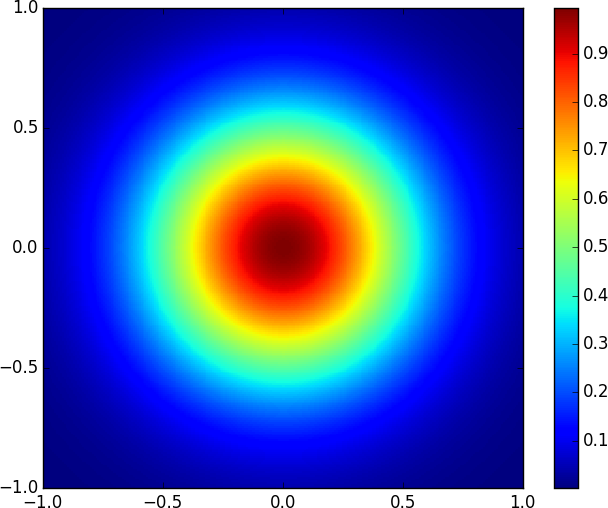
\includegraphics[width=\textwidth]{initcond_gaussian.png}

            \column{0.33 \textwidth}
            \centering
            $\sigma_T$ for Lattice Initial Condition

            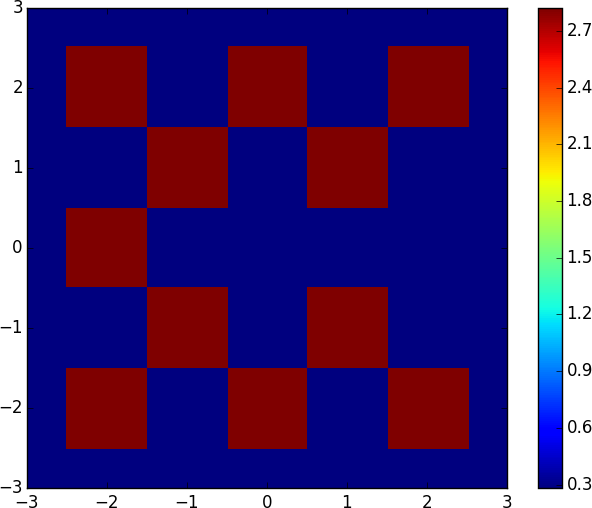
\includegraphics[width=\textwidth]{initcond_lattice-t.png}

            \column{0.33 \textwidth}
            \centering
            Smooth Initial Condition

            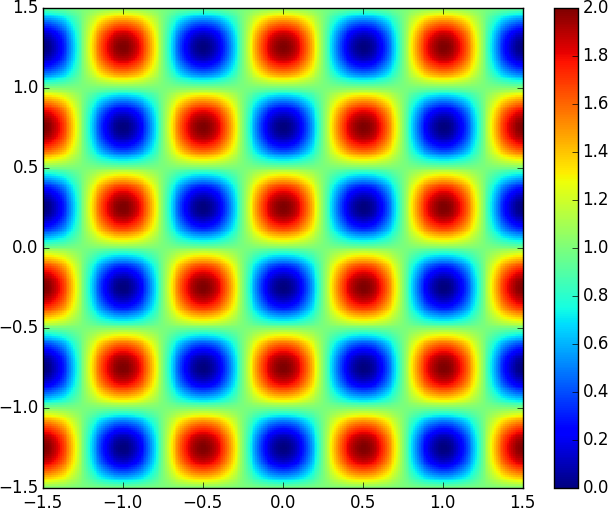
\includegraphics[width=\textwidth]{initcond_smooth.png}
        \end{columns}
    \end{frame}

    \begin{frame}{Time Stepping}
        \begin{block}{CFL Condition}
            A small enough time step is necessary for convergence. In this case,
            \begin{equation*}
                \frac{\Delta t}{\Delta x} + \frac{\Delta t}{\Delta y} \leq 1
            \end{equation*}
        \end{block}

        \vfill

        \begin{block}{Heun's Method}
            To compute a first estimate, carry out two Euler steps.
            Now use the average of the initial state and the estimate.
            \begin{itemize}
                \item Explicit, two-stage Runge-Kutta method
                \item Second order accurate
                \item Strong stability preserving
            \end{itemize}
        \end{block}
    \end{frame}

    \begin{frame}{Quadratures}
        Currently uses Chebyshev-Legendre quadrature.
        \begin{itemize}
            \item Constructed from $n$ Gauss-Legendre rule
            \item Optimized for symmetry
            \item Exactly integrates to order $2n - 1$ moments
        \end{itemize}

        \vfill

        Added (experimental) Lebedev quadrature
        \begin{itemize}
            \item Constructed based on octahedral symmetry group
            \item Optimal with respect to number of points
            \item Structure does not lend itself to symmetry optimizations
            \item Negative weights
        \end{itemize}
    \end{frame}

    \begin{frame}{Optimization Problem}
        \momopt uses nonlinear spectral methods, so updates entail solving an optimiztion problem for a given \vec{u} and moments \vec{m}.
        \begin{equation*}
            \min_{\vec{\alpha}} \integral{\exp(\T{\vec{\alpha}} \vec{m})} - \T{\vec{\alpha}} \vec{u}
        \end{equation*}

        \vfill

        To use a Newton solver, we need
        \begin{itemize}
            \item An objective funtion $F(\vec{\alpha}) = \integral{\exp(\T{\vec{\alpha}} \vec{m})} - \T{\vec{\alpha}} \vec{u}$
            \item Gradient $g(\vec{\alpha})$ of $F(\vec{\alpha})$
            \item Hessian $H(\vec{\alpha})$ of $F(\vec{\alpha})$
        \end{itemize}

        \vfill

        Now the estimated $\vec{\alpha}' = \vec{\alpha} + t\vec{d}$ where $\vec{d} = -H(\vec{\alpha})^{-1}g(\vec{\alpha})$.
    \end{frame}

    \begin{frame}{$\gamma$ factor}
        \momopt computes ansatz for the optimization, yielding an \emph{approximate} solution $\vec{u} \approx \integral{\exp (\T{\vec{\alpha}})}$.

        Needed to estimate error and try to correct via $\gamma$ ratio.

        Required fine mesh and low tolerance on optimization to prevent non-realizability.

        Instead, compute $\hat{\vec{u}}$ such that $\hat{\vec{u}} = \integral{\exp \left(\T{\vec{\alpha}}\right)}$.
    \end{frame}

    \begin{frame}{Fixed regularization}
        In case of bad condition number (i.e. the system is too sensitive to errors) fall back to isotropic \vec{\alpha} to allow the algorithm to complete successfully
    \end{frame}

    \begin{frame}{Source Code}
        The source code is available on Github

        \url{https://github.com/ckrisgarrett/closures-2d}
    \end{frame}

    \begin{frame}{Bibliography}
        cite that presentation, linesource paper
    \end{frame}
\end{document}
